\documentclass[12pt,a4paper]{report}

% ===================== PACKAGES =====================
\usepackage[utf8]{inputenc}
\usepackage[T5]{fontenc}
\usepackage[vietnamese]{babel}
\usepackage{geometry}
\usepackage{graphicx}
\usepackage{hyperref}
\usepackage{tocloft}
\usepackage{booktabs}
\usepackage{array}
\usepackage{longtable}
\usepackage{tabularx}
\usepackage{enumitem}
\usepackage{setspace}
\usepackage{titlesec}
\usepackage{fancyhdr}
\usepackage{caption}
\usepackage{float}
\usepackage{xcolor}
\usepackage{amsmath}
\usepackage{indentfirst}
\usepackage{tikz}
\usepackage{pgfornament}
\usepackage{xurl}
\usepackage{hyperref}
\hypersetup{breaklinks=true} 

% ===================== PAGE LAYOUT =====================
\geometry{
    a4paper,
    top=2.5cm,
    bottom=2.5cm,
    left=3cm,
    right=2cm
}

% ===================== HYPERLINKS =====================
\hypersetup{
    colorlinks=true,
    linkcolor=black,
    urlcolor=blue,
    citecolor=black,
    pdftitle={Báo Cáo Cuối Kì - Hệ Thống Tưới Cây Thông Minh},
    pdfauthor={Nhóm D22CNPM02}
}

% ===================== HEADER/FOOTER =====================
\pagestyle{fancy}
\fancyhf{}
\fancyhead[R]{\small Hệ thống tưới cây thông minh}
\fancyfoot[C]{\thepage}
\renewcommand{\headrulewidth}{0.4pt}

% ===================== SECTION FORMATTING =====================
\titleformat{\chapter}[block]
  {\normalfont\large\bfseries\centering}
  {\Roman{chapter}.}{0.5em}{}
\titlespacing*{\chapter}{0pt}{10pt}{15pt}

\titleformat{\section}
  {\normalfont\normalsize\bfseries}
  {\thesection}{0.5em}{}
\titlespacing*{\section}{0pt}{10pt}{6pt}

\titleformat{\subsection}
  {\normalfont\normalsize\bfseries}
  {\thesubsection}{0.5em}{}
\titlespacing*{\subsection}{0pt}{8pt}{4pt}

\titleformat{\subsubsection}
  {\normalfont\normalsize\itshape}
  {\thesubsubsection}{0.5em}{}

% ===================== TOC SETTINGS =====================
\renewcommand{\contentsname}{MỤC LỤC}
\renewcommand{\listfigurename}{DANH MỤC HÌNH ẢNH}
\renewcommand{\listtablename}{DANH MỤC BẢNG BIỂU}

\setlength{\cftbeforetoctitleskip}{0pt}
\setlength{\cftbeforeloftitleskip}{0pt}

% ===================== LINE SPACING =====================
\onehalfspacing

% ===================== CAPTION SETTINGS =====================
\captionsetup{
    font=small,
    labelfont=bf,
    labelsep=period,
    justification=centering
}

% ===================== DOCUMENT =====================
\begin{document}

\begin{titlepage}
    % ====== FRAME ONLY FOR COVER PAGE ======
    \begin{tikzpicture}[remember picture,overlay]

        % Outer border (blue)
        \draw[black!70!black, line width=1.2pt]
          ([xshift=10mm,yshift=-10mm]current page.north west)
          rectangle
          ([xshift=-10mm,yshift=10mm]current page.south east);

        % Inner border (blue)
        \draw[black!70!black, line width=0.8pt]
          ([xshift=13mm,yshift=-13mm]current page.north west)
          rectangle
          ([xshift=-13mm,yshift=13mm]current page.south east);

        % Corner ornaments (black/gray like sample)
        \node[anchor=north west] at ([xshift=12.5mm,yshift=-12.5mm]current page.north west)
          {\pgfornament[width=18mm,color=black!70]{61}};
        \node[anchor=north east] at ([xshift=-12.5mm,yshift=-12.5mm]current page.north east)
          {\pgfornament[width=18mm,color=black!70,symmetry=v]{61}};
        \node[anchor=south west] at ([xshift=12.5mm,yshift=12.5mm]current page.south west)
          {\pgfornament[width=18mm,color=black!70,symmetry=h]{61}};
        \node[anchor=south east] at ([xshift=-12.5mm,yshift=12.5mm]current page.south east)
          {\pgfornament[width=18mm,color=black!70,symmetry=c]{61}};

    \end{tikzpicture}

    \thispagestyle{empty}
    \begin{center}
        \textbf{\large HỌC VIỆN CÔNG NGHỆ BƯU CHÍNH VIỄN THÔNG}\\[0.3cm]
        \textbf{\large KHOA CÔNG NGHỆ THÔNG TIN 1}\\[1cm]

        % Logo (nếu có file ảnh logo, thay đường dẫn tương ứng)
        
\includegraphics[width=4cm]{logo.png}

        \vspace{1cm}
        \textbf{\LARGE BÁO CÁO CUỐI KÌ}\\[0.5cm]
        \textbf{\Large HỌC PHẦN HỆ THỐNG NHÚNG}\\[1cm]

        \textbf{Lớp chuyên ngành: D22CNPM02}\\[1cm]

        \textbf{\Large ĐỀ TÀI: HỆ THỐNG TƯỚI CÂY THÔNG MINH}\\[1cm]

        \textbf{Giảng viên hướng dẫn: TS. Phạm Hoàng Việt}\\[1cm]

        \textbf{Danh sách thành viên nhóm:}\\[0.5cm]
        \begin{tabular}{ll}
            Phan Văn Thuỷ   & B22DCCN844 \\
            Lê Vũ Thành Vinh & B22DCCN904 \\
            Bùi Văn Hiến     & B22DCCN292 \\
            Hoàng Việt Anh   & B22DCCN017 \\
            Trần Đức Phương  & B22DCCN640 \\
        \end{tabular}

        \vfill
        \textbf{Hà Nội, 2026}
    \end{center}
\end{titlepage}

% ========== MỤC LỤC ==========
\cleardoublepage
\tableofcontents

% ========== DANH MỤC HÌNH ẢNH ==========
\cleardoublepage
\listoffigures

% ========== NỘI DUNG CHÍNH ==========
\cleardoublepage
\pagenumbering{arabic}
\setcounter{page}{1}

% ============================================================
\chapter{GIỚI THIỆU ĐỀ TÀI}
% ============================================================

\section{Bối cảnh và lý do chọn đề tài}

\subsection*{a. Bối cảnh thực tế}

Trong bối cảnh đô thị hóa và nông nghiệp công nghệ cao đang phát triển
mạnh mẽ, nhu cầu chăm sóc cây xanh -- từ cây cảnh trong gia đình, văn
phòng đến các mô hình nông nghiệp đô thị -- ngày càng gia tăng.
Tuy nhiên, thực tế cho thấy:

\begin{itemize}
    \item \textbf{Sự đa dạng về nhu cầu sinh lý của cây trồng:} Mỗi loại cây
    (xương rồng, nha đam, tía tô,\ldots) có nhu cầu về lượng nước, tần suất tưới
    và độ ẩm đất hoàn toàn khác nhau. Việc tưới cùng một chế độ cho mọi loại cây
    dẫn đến cây bị úng hoặc khô héo.

    \item \textbf{Hạn chế của các giải pháp tưới tự động hiện có:} Các bộ hẹn giờ
    cơ học hoặc cảm biến độ ẩm đơn thuần chỉ tưới theo ngưỡng cài đặt sẵn, không
    thể phân biệt được đang tưới cho cây gì. Ví dụ: cây xương rồng cần đất khô
    hoàn toàn trước khi tưới.

    \item \textbf{Thiếu sự cá nhân hóa và thích ứng:} Người dùng không phải lúc
    nào cũng có kiến thức chuyên sâu về từng loại cây. Hệ thống hiện tại không thể
    tự động ``học'' và điều chỉnh chế độ tưới phù hợp khi thay đổi chậu cây hoặc
    trồng loại cây mới.

    \item \textbf{Bài toán đặt ra:} Làm thế nào để xây dựng một hệ thống tưới cây
    thông minh, có khả năng ``nhìn'' và ``nhận biết'' chính xác loại cây đang được
    chăm sóc, từ đó tự động tra cứu và áp dụng chế độ tưới tối ưu, đảm bảo cây
    phát triển tốt nhất mà không cần sự can thiệp thủ công của con người?
\end{itemize}

\subsection*{b. Động lực và ý nghĩa của đề tài}

Đề tài ``Hệ thống tưới cây tự động tích hợp AI nhận diện loại cây'' hướng
đến phân khúc IoT Smart Garden (Vườn thông minh) và Robotics trong nông nghiệp
hộ gia đình. Động lực chính bao gồm:

\begin{itemize}
    \item \textbf{Tối ưu hóa tài nguyên nước:} Tưới đúng lượng, đúng thời điểm
    giúp tiết kiệm nước -- một vấn đề cấp bách trong bối cảnh biến đổi khí hậu.

    \item \textbf{Nâng cao trải nghiệm người dùng:} Giải phóng sức lao động,
    giảm gánh nặng ghi nhớ lịch tưới cho từng loại cây, đặc biệt hữu ích cho
    người bận rộn hoặc người cao tuổi.

    \item \textbf{Ứng dụng công nghệ AI biên (Edge AI):} Thay vì gửi ảnh lên
    cloud để xử lý (gây độ trễ, mất an toàn dữ liệu), hệ thống tích hợp mô hình
    học sâu nhẹ chạy trực tiếp trên vi điều khiển như ESP32-CAM, đảm bảo nhận
    diện cây theo thời gian thực ngay tại vườn.
\end{itemize}

\section{Khảo sát và lựa chọn công nghệ}

Để đảm bảo tính khả thi và đúng đắn cho hệ thống nhúng, nhóm đã khảo sát
ba hướng tiếp cận chính và lựa chọn phương án tối ưu:

\begin{longtable}{|p{2.5cm}|p{3cm}|p{2.5cm}|p{3cm}|p{2.5cm}|}
\hline
\textbf{Phương án} & \textbf{Mô tả} & \textbf{Ưu điểm} & \textbf{Nhược điểm} & \textbf{Kết luận} \\
\hline
\endfirsthead
\hline
\textbf{Phương án} & \textbf{Mô tả} & \textbf{Ưu điểm} & \textbf{Nhược điểm} & \textbf{Kết luận} \\
\hline
\endhead
1. Nhận diện qua Cloud (Google Vision API) &
Gửi ảnh từ camera lên server qua Wi-Fi, nhận kết quả loại cây. &
Độ chính xác cao, không yêu cầu phần cứng mạnh. &
Phụ thuộc hoàn toàn vào Internet, độ trễ cao (vài giây), chi phí vận hành, lo ngại về quyền riêng tư. &
Không phù hợp do yêu cầu real-time và hoạt động ổn định ngoại vi. \\
\hline
2. Cảm biến đa phổ + Thuật toán truyền thống &
Sử dụng cảm biến màu sắc/độ phản xạ ánh sáng để phân loại cây theo dạng lá. &
Không cần xử lý ảnh phức tạp, tiêu tốn ít năng lượng. &
Chỉ phân biệt được cây có màu sắc rất khác biệt, không nhận diện được chủng loại cây cùng màu xanh. &
Không đủ thông minh cho bài toán đa dạng các loại cây. \\
\hline
3. AI biên (TinyML) trên Vi điều khiển &
Chạy mô hình CNN (ví dụ MobileNetV1) đã được lượng tử hóa trên ESP32-CAM (240 MHz, 520 KB RAM). &
Độ trễ thấp ($\sim$100--300 ms), bảo mật dữ liệu, chi phí phần cứng thấp ($<$500k VNĐ). &
Yêu cầu tối ưu mô hình mạnh (dùng TensorFlow Lite Micro), độ chính xác có thể giảm nhẹ so với cloud. &
\textbf{Lựa chọn tối ưu} -- Đáp ứng đúng đặc thù của hệ thống nhúng. \\
\hline
\caption{So sánh các phương án công nghệ}
\end{longtable}

\textbf{Lý do kỹ thuật chọn phương án 3:}

\begin{itemize}
    \item \textbf{Vi điều khiển:} Sử dụng ESP32-CAM (SoC Xtensa LX6 240MHz,
    520KB SRAM, hỗ trợ camera OV2640). Đây là nền tảng phổ biến, mạnh mẽ cho
    các bài toán xử lý ảnh nhúng, có sẵn thư viện camera và hỗ trợ TensorFlow
    Lite Micro.

    \item \textbf{Mô hình AI:} Huấn luyện mô hình MobileNetV1 (phiên bản 0.25x)
    trên tập dữ liệu ảnh lá cây (xương rồng, nha đam, tía tô\ldots). Sau đó,
    lượng tử hóa (quantization) từ float32 xuống int8, giảm kích thước từ 14 MB
    xuống còn $\sim$250 KB, phù hợp với bộ nhớ Flash của ESP32.
\end{itemize}

% ============================================================
\chapter{NỘI DUNG CHÍNH}
% ============================================================

\section{Yêu cầu đối với hệ thống cần xây dựng}

\subsection{Sơ đồ thiết kế hệ thống}

\begin{figure}[H]
    \centering
    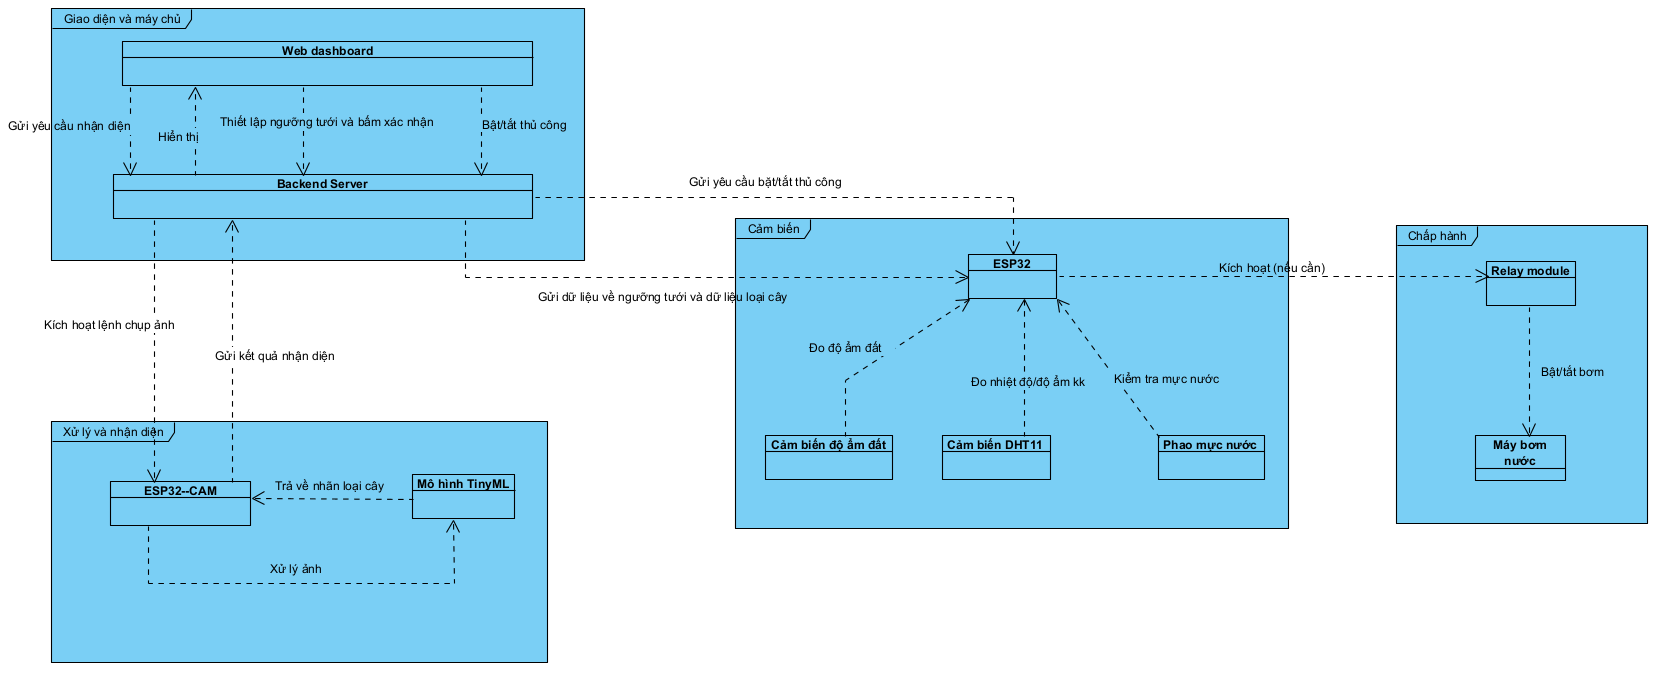
\includegraphics[width=1.1\textwidth]{image1.png}
    \caption{Sơ đồ thiết kế hệ thống}
    \label{fig:system-design}
\end{figure}

\textbf{Nhận diện loại cây:}
\begin{itemize}
    \item Người dùng bấm nút nhận diện loại cây trên giao diện web, yêu cầu được
    gửi đến backend.
    \item Backend gọi đến ESP32-CAM để thực hiện chụp ảnh và nhận diện.
    \item Kết quả được trả lại cho backend và hiển thị lên giao diện.
    \item Người dùng thiết lập ngưỡng tưới cho loại cây đó và bấm xác nhận.
    \item Dữ liệu về ngưỡng tưới và thông tin về loại cây được gửi đến ESP32.
    \item ESP32 thu thập dữ liệu từ môi trường và kết hợp với dữ liệu được gửi từ
    backend để đưa ra yêu cầu tưới.
    \item ESP32 kích hoạt máy bơm để bật nếu cần.
\end{itemize}

\textbf{Bật/tắt thủ công:}
\begin{itemize}
    \item Người dùng bấm nút bật/tắt trên giao diện.
    \item Yêu cầu được gửi đến ESP32.
    \item ESP32 kích hoạt bơm nếu cần.
\end{itemize}

\subsection{Yêu cầu chức năng}

\begin{itemize}
    \item \textbf{Nhận diện loại cây:} ESP32-CAM phải chụp ảnh và phân loại được
    loại cây (nha đam, xương rồng, tía tô).
    \item \textbf{Tự động điều chỉnh ngưỡng tưới:} Tùy vào loại cây đã nhận diện,
    hệ thống phải tự động thay đổi ngưỡng độ ẩm.
    \item \textbf{Giám sát độ ẩm đất:} Cảm biến độ ẩm đất phải hoạt động liên tục
    để cung cấp dữ liệu thời gian thực cho ESP32.
    \item \textbf{Điều khiển máy bơm:} Relay phải kích hoạt máy bơm khi độ ẩm dưới
    ngưỡng và tự động ngắt khi đạt ngưỡng.
    \item \textbf{Bảo vệ cạn nước:} Phao cảm biến điện tử phải kiểm tra mực nước
    trong bình chứa. Nếu hết nước, hệ thống không được bật bơm và phải phát cảnh báo.
    \item \textbf{Chế độ thủ công:} Cho phép người dùng bật/tắt bơm thông qua nút
    bấm trên giao diện web.
\end{itemize}

\subsection{Yêu cầu phi chức năng}

\begin{itemize}
    \item \textbf{Độ chính xác nhận diện:} Mô hình AI chạy trên ESP32-CAM đạt độ
    chính xác tối thiểu 70\%.
    \item \textbf{Thời gian phản hồi:} Từ lúc cảm biến nhận thấy đất khô đến lúc
    bơm bật không quá 3 giây. Thời gian nhận diện hình ảnh không quá 7 giây.
\end{itemize}

% ============================================================
\section{Các thành phần phần cứng}

\subsection{Module ESP32}

\subsubsection{Giới thiệu chung}

\begin{figure}[H]
    \centering
    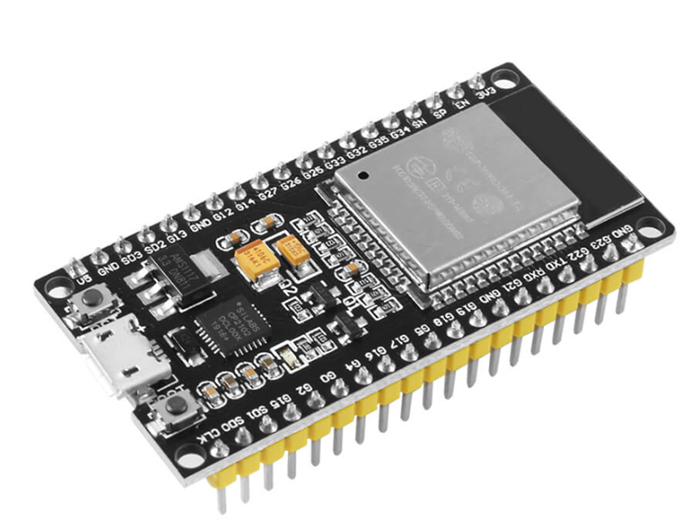
\includegraphics[width=0.55\textwidth]{image2.png}
    \caption{Module ESP32}
    \label{fig:esp32}
\end{figure}

ESP32 là một dòng chip vi điều khiển được phát triển bởi Espressif, với nhiều
đặc điểm ưu việt:

\begin{itemize}
    \item \textbf{Giá rẻ:} So với các dòng vi điều khiển khác, ESP32 có giá thành
    phải chăng hơn rất nhiều, giúp tất cả những ai đam mê công nghệ có thể dễ
    dàng tiếp cận.

    \item \textbf{Lượng điện tiêu thụ thấp:} ESP32 tiêu thụ rất ít năng lượng.
    Dòng chip này cũng hỗ trợ các trạng thái tiết kiệm năng lượng như Deep Sleep để tiết kiệm điện.

    \item \textbf{Có thể kết nối Wi-Fi:} Có thể dễ dàng kết nối ESP32 với mạng
    Wi-Fi để truy cập Internet (chế độ trạm -- Station mode) hoặc tạo một mạng
    WiFi riêng nó (chế độ điểm truy cập -- Access point) để các thiết bị khác có thể kết nối với nó. Chế độ Access point thường được dùng trong các dự án IoT hoặc tự động hóa trong Smart Home, trong đó có thể cho phép nhiều thiết bị liên lạc và trao đổi thông tin với nhau thông qua WiFi của chúng.

    \item \textbf{Hỗ trợ Bluetooth:} ESP32 hỗ trợ cả Bluetooth Classic và
    Bluetooth Low Energy (BLE)– một công cụ rất hữu ích cho những ứng dụng IoT.

    \item \textbf{Lõi kép:} Đa số các dòng chip ESP32 hiện nay đều có lõi kép,
    đi kèm với 2 bộ vi xử lý Xtensa 32-bit LX6.

    \item \textbf{Đa dạng thiết bị ngoại vi:} ESP32 hỗ trợ nhiều loại thiết bị
    ngoại vi như cảm ứng điện dung, I2C, DAC, PWM, UART, SPI,\ldots

    \item \textbf{Tương thích với Arduino và MicroPython:} ESP32 có thể được lập
    trình bằng ngôn ngữ Arduino và MicroPython.
\end{itemize}

\textbf{Thông số kỹ thuật:}

\textit{1. Kết nối không dây}
\begin{itemize}
    \item WiFi: Tốc độ dữ liệu lên đến 150Mbps với HT40.
    \item Bluetooth: Hỗ trợ BLE (Bluetooth Low Energy) và Bluetooth Classic.
    \item Bộ xử lý: Chip vi xử lý LX6 32-bit Tensilica Xtensa Dual-Core, hoạt
    động ở tốc độ 160MHz hoặc 240MHz.
\end{itemize}

\textit{2. Bộ nhớ}
\begin{itemize}
    \item \textbf{ROM:} 448 KB (phục vụ cho việc khởi động và chạy các chức năng
    cốt lõi).
    \item \textbf{SRAM:} 520 KB (dùng cho dữ liệu và hướng dẫn).
    \item \textbf{RTC fast SRAM:} 8 KB (dùng để lưu trữ dữ liệu trong chế độ
    Deep Sleep).
    \item \textbf{RTC slow SRAM:} 8 KB (dùng để truy cập bộ đồng xử lý trong
    chế độ Deep Sleep).
    \item \textbf{eFuse:} 1 Kbit, trong đó 256 bit phục vụ cho hệ thống (địa chỉ
    MAC và cấu hình chip), 768 bit còn lại dành cho ứng dụng người dùng.
    \item \textbf{Embedded flash:}
    \begin{itemize}
        \item 0 MiB (ESP32-D0WDQ6, ESP32-D0WD, and ESP32-S0WD chips)
        \item 2 MiB (ESP32-D2WD chip)
        \item 4 MiB (ESP32-PICO-D4 SiP module)
    \end{itemize}
\end{itemize}

\textit{3. Công suất}

ESP32 cho phép vẫn có thể sử dụng bộ chuyển đổi ADC, kể cả khi đang trong
chế độ Deep Sleep.

\textit{4. Hỗ trợ các thiết bị ngoại vi đầu ra / đầu vào}
\begin{itemize}
    \item Giao diện ngoại vi với DMA bao gồm cảm ứng điện dung.
    \item ADC (Analog to Digital Converter).
    \item DAC (Digital to Analog Converter).
    \item I2C (Inter Integrated Circuit).
    \item UART (Universal Asynchronous Receiver/Transmitter).
    \item SPI (Serial Peripheral Interface).
    \item I2S (Integrated Interchip Sound).
    \item RMII (Reduced Media-Independent Interface).
    \item PWM (Pulse-Width Modulation).
\end{itemize}

\textit{5. Tính bảo mật}

Bộ tăng tốc phần cứng dành cho SSL/TLS và AES.

\subsubsection{Nguyên lý hoạt động}

Nguyên lý hoạt động của ESP32 dựa trên việc kết hợp bộ xử lý lõi kép mạnh
mẽ, tích hợp Wi-Fi và Bluetooth, cho phép xử lý dữ liệu, kết nối mạng và
giao tiếp với các thiết bị ngoại vi khác thông qua nhiều giao thức như ADC,
SPI, I2C, UART. ESP32 nhận tín hiệu từ các cảm biến và xử lý chúng, sau đó
thực hiện các tác vụ như kết nối mạng, gửi dữ liệu lên đám mây hoặc điều
khiển các thiết bị khác.

% ============================================================
\subsection{Cảm biến độ ẩm đất điện dung}

\subsubsection{Giới thiệu chung}

\begin{figure}[H]
    \centering
    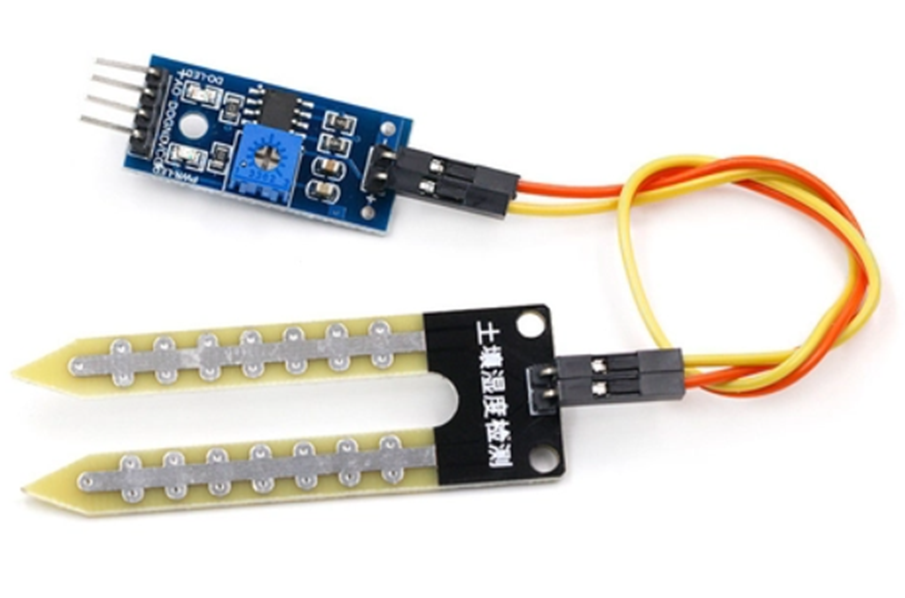
\includegraphics[width=0.6\textwidth]{image3.png}
    \caption{Cảm biến độ ẩm đất}
    \label{fig:soil-sensor}
\end{figure}

Cảm biến độ ẩm đất Soil Moisture Sensor là thiết bị điện tử được sử dụng để
đo lượng nước trong đất, giúp theo dõi tình trạng độ ẩm của đất và hỗ trợ
các ứng dụng nông nghiệp, trồng trọt, và hệ thống tưới tiêu tự động.

\textbf{Thông số kỹ thuật:}
\begin{itemize}
    \item Điện áp hoạt động: 3.3V -- 5V.
    \item Kích thước PCB: 3cm $\times$ 1.6cm.
    \item Led đỏ báo nguồn vào, Led xanh báo độ ẩm.
    \item IC so sánh: LM393.
    \item VCC: 3.3V -- 5V.
    \item GND: 0V.
    \item DO: Đầu ra tín hiệu số (0 và 1).
    \item AO: Đầu ra Analog (tín hiệu tương tự).
\end{itemize}

\subsubsection{Nguyên lý hoạt động}

\begin{figure}[H]
    \centering
    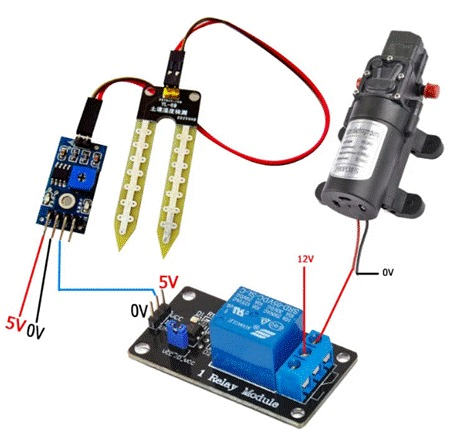
\includegraphics[width=0.6\textwidth]{image4.png}
    \caption{Ví dụ hệ thống tưới nước sử dụng cảm biến độ ẩm đất}
    \label{fig:soil-watering-example}
\end{figure}

\begin{itemize}
    \item Khi đất khô, module cảm biến đưa ra chân D0 mức 1. Module relay không
    hoạt động nên bơm hoạt động.
    \item Khi nước đủ ẩm, chân D0 xuống mức 0, module Rơle hoạt động nên bơm
    không hoạt động.
\end{itemize}

% ============================================================
\subsection{Relay module}

\subsubsection{Giới thiệu chung}

\begin{figure}[H]
    \centering
    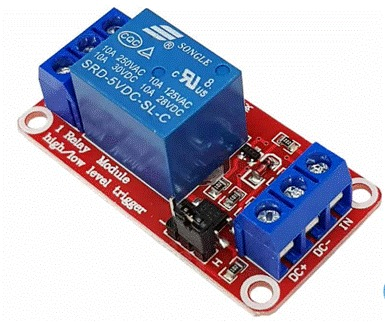
\includegraphics[width=0.5\textwidth]{image5.png}
    \caption{Relay module}
    \label{fig:relay}
\end{figure}

Relay là một công tắc điện từ hoạt động nhờ vào một dòng điện nhỏ, có khả
năng bật hoặc tắt một dòng điện lớn hơn nhiều lần. Trái tim của relay là
cuộn dây điện (hay còn gọi là nam châm điện) -- khi có dòng điện chạy qua,
cuộn dây sẽ tạo ra một từ trường, khiến nó trở thành một nam châm tạm thời. Từ đó, relay có thể đóng mở các tiếp điểm điện, giúp điều khiển dòng điện lớn hơn.

\textbf{Cấu tạo của relay} bao gồm 3 phần chính:
\begin{itemize}
    \item \textbf{Khối tiếp nhận:} Nhận tín hiệu đầu vào và chuyển đổi nó thành
    tín hiệu thích hợp để truyền đến khối trung gian.
    \item \textbf{Khối trung gian:} Tiếp nhận tín hiệu từ khối tiếp nhận và
    chuyển đổi nó thành tín hiệu điều khiển cho relay.
    \item \textbf{Khối chấp hành:} Thực hiện tác động vào mạch điều khiển, giúp
    relay đóng hoặc mở các tiếp điểm điện.
\end{itemize}

\textbf{Thông số kỹ thuật:}
\begin{itemize}
    \item \textbf{Hiệu điện thế kích tối ưu:} Đây là yếu tố quyết định việc relay
    có hoạt động đúng hay không. Ví dụ, nếu cần điều khiển một bóng đèn 220V từ
    một cảm biến ánh sáng hoạt động ở mức 5 -- 12V, sẽ cần một module relay có
    hiệu điện thế kích là 5V hoặc 12V.
    \item \textbf{Hiệu điện thế và cường độ dòng điện tối đa:} Thông số này cho
    biết mức dòng điện và điện áp tối đa mà relay có thể chịu đựng.
\end{itemize}

\subsubsection{Nguyên lý hoạt động}

\begin{itemize}
    \item Điện được cấp cho cuộn dây, tạo ra từ trường.
    \item Từ trường tác động lên phần ứng, tạo ra lực hút.
    \item Phần ứng di chuyển, đóng hoặc mở các tiếp điểm điện.
    \item Các tiếp điểm chuyển mạch dòng điện đến các thiết bị như động cơ,
    bóng đèn, v.v.
    \item Khi điện áp bị loại bỏ, từ trường biến mất và các tiếp điểm trở lại
    vị trí ban đầu.
\end{itemize}

% ============================================================
\subsection{Máy bơm nước}

\subsubsection{Giới thiệu chung}

\begin{figure}[H]
    \centering
    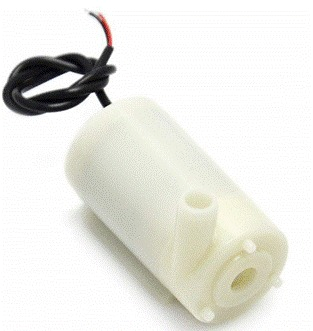
\includegraphics[width=0.4\textwidth]{image6.png}
    \caption{Máy bơm nước}
    \label{fig:water-pump}
\end{figure}

Động cơ bơm chìm Mini Water Pump 5VDC có kích thước rất nhỏ gọn, sử dụng
điện áp 3$\sim$5VDC, thuộc dạng bơm chìm nên động cơ có khả năng chống nước và
hoạt động khi ngâm chìm trong nước, ứng dụng để bơm nước, dung dịch trong
các thiết kế nhỏ, mô hình tưới cây, hồ cá,\ldots

\textbf{Thông số kỹ thuật:}
\begin{itemize}
    \item Điện áp sử dụng: 3$\sim$5VDC.
    \item Dòng điện sử dụng: 100$\sim$200mA.
    \item Lưu lượng bơm: 1.2$\sim$1.6L / 1 phút.
    \item Đường kính ngoài ống dẫn: 7.5mm.
    \item Kích thước: 34 $\times$ 43 mm.
    \item Trọng lượng: 28g.
\end{itemize}

\subsubsection{Nguyên lý hoạt động}

Máy bơm mini IoT hoạt động bằng cách kết hợp nguyên lý hoạt động của máy
bơm nước truyền thống và công nghệ Internet of Things (IoT) để điều khiển từ
xa. Máy bơm sẽ hoạt động khi áp suất nước giảm dưới ngưỡng cài đặt, và ngừng
lại khi áp suất đạt mức mong muốn, với tín hiệu từ cảm biến được xử lý qua
mạng internet để ra lệnh cho động cơ máy bơm thông qua một bộ điều khiển và
relay.

% ============================================================
\subsection{Module ESP32-CAM}

\subsubsection{Giới thiệu chung}

\begin{figure}[H]
    \centering
    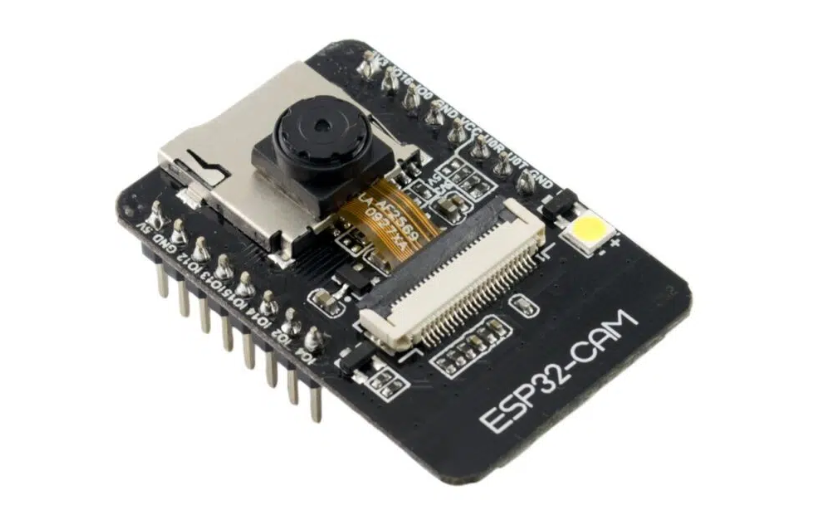
\includegraphics[width=0.65\textwidth]{image7.png}
    \caption{Module ESP32-CAM}
    \label{fig:esp32-cam}
\end{figure}

ESP32-CAM có một camera kích thước nhỏ, giống như mô-đun chính, mô-đun này có
thể được xử lý công việc độc lập, có kích thước nhỏ gọn chỉ 40 $\times$ 27 $\times$
12 mm, dòng nghỉ chỉ 6mA.

ESP32-CAM có thể được sử dụng rộng rãi trong các ứng dụng IoT khác nhau, thích
hợp cho thiết bị thông minh gia đình, điều khiển không dây công nghiệp, giám
sát không dây kiểm soát, nhận dạng không dây QR, tín hiệu hệ thống định vị
không dây.

\textbf{Thông số kỹ thuật:}
\begin{itemize}
    \item IC chính: ESP32-S (AI-Thinker).
    \item Mô-đun Wi-Fi BT SoC 802.11 b/g/n/e/i.
    \item CPU 32-bit công suất thấp.
    \item Tốc độ đồng hồ lên đến 160MHz, sức mạnh tính toán lên đến 600 DMIPS.
    \item Tích hợp 520 KB SRAM, 4MB PSRAM bên ngoài.
    \item Dải tần số: 1421 $\sim$ 2484 MHz.
    \item Bluetooth: 4.2 BR/EDR BLE.
    \item Hỗ trợ UART / SPI / I2C / PWM / ADC / DAC.
    \item Hỗ trợ máy ảnh OV2640 và OV7670, đèn flash tích hợp.
    \item Hỗ trợ tải lên WiFi hình ảnh.
    \item Hỗ trợ thẻ TF.
    \item Hỗ trợ nhiều chế độ ngủ.
    \item Nhúng Lwip và FreeRTOS.
    \item Hỗ trợ chế độ hoạt động STA / AP / STA + AP.
    \item Hỗ trợ cấu hình thông minh / công nghệ AirKiss.
    \item Hỗ trợ nâng cấp cục bộ và từ xa cho cổng nối tiếp (FOTA).
\end{itemize}

\subsubsection{Nguyên lý hoạt động}

ESP32-CAM là mô-đun camera Wi-Fi/Bluetooth nhỏ gọn dựa trên chip ESP32-S, hoạt
động bằng cách chụp ảnh qua cảm biến OV2640/OV7670, xử lý dữ liệu qua vi xử
lý 32-bit (lên đến 160MHz) và truyền hình ảnh qua WiFi hoặc lưu vào thẻ SD.

% ============================================================
\subsection{Phao điện tử cảm biến mực nước}

\subsubsection{Giới thiệu chung}

Phao cảm biến mực nước là loại công tắc từ, bình thường hai tiếp điểm của
phao khi hướng xuống sẽ ở trạng thái đóng (NC), khi có mực chất lỏng làm
phao nổi lên sẽ chuyển thành trạng thái mở (NO), dựa vào đặc tính này phao
điện từ được sử dụng cho các ứng dụng: cảnh báo mực chất lỏng, báo đầy,\ldots

\begin{figure}[H]
    \centering
    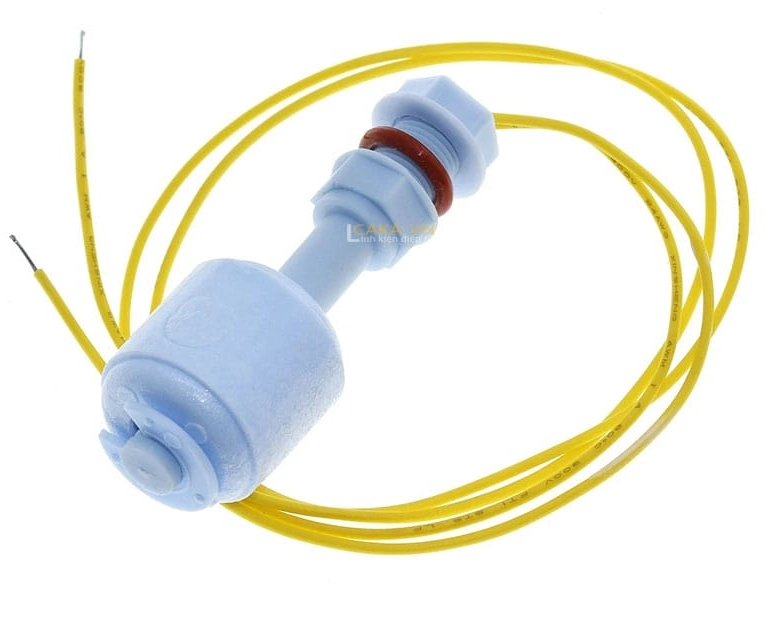
\includegraphics[width=0.55\textwidth]{image8.png}
    \caption{Phao cảm biến điện tử}
    \label{fig:water-level-sensor}
\end{figure}

\textbf{Thông số kỹ thuật:}
\begin{itemize}
    \item Chiều dài tổng: 52mm.
    \item Loại: Phao cảm biến mực nước dạng ngang.
    \item Chất liệu: Nhựa PP (chống ăn mòn, dùng tốt với nước sạch).
    \item Ngõ ra: 2 dây (công tắc từ -- thường đóng hoặc thường mở).
    \item Điện áp chịu tải: tối đa 100VDC.
    \item Dòng điện tối đa: 0.5A.
    \item Khoảng cách lắp đặt: gắn thành bể, đường kính lỗ lắp 8$\sim$10mm.
    \item Nhiệt độ hoạt động: $-10^{\circ}$C đến $+85^{\circ}$C.
    \item Độ kín nước: IP65 trở lên.
    \item Nguyên lý hoạt động: khi nước chạm đến phao $\rightarrow$ phao nổi
    $\rightarrow$ công tắc đóng/mở tùy chiều lắp.
\end{itemize}

\subsubsection{Nguyên lý hoạt động}

Phao cảm biến mực nước 52mm là công tắc từ tính dạng nằm ngang, hoạt động theo
nguyên lý nam châm bên trong phao tác động lên công tắc reed khi mực nước thay
đổi. Thiết bị có thể phát hiện nước đầy hoặc cạn, thường được lắp trong bể nước,
bình chứa, máy lọc nước, bể cá, hoặc các hệ thống bơm tự động.

% ============================================================
\subsection{Cảm biến nhiệt độ, độ ẩm không khí DHT11}

\subsubsection{Giới thiệu chung}

\begin{figure}[H]
    \centering
    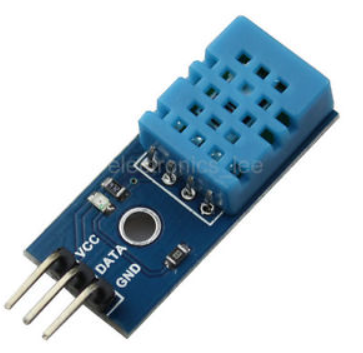
\includegraphics[width=0.45\textwidth]{image9.png}
    \caption{Cảm biến nhiệt độ, độ ẩm không khí DHT11}
    \label{fig:dht11}
\end{figure}

DHT11 là một cảm biến đo nhiệt độ và độ ẩm kỹ thuật số đơn giản và giá thành
rất rẻ, được sử dụng phổ biến trong các ứng dụng đo lường môi trường cơ bản.
Cảm biến này sử dụng một cảm biến độ ẩm điện dung và một điện trở nhiệt
(thermistor) để đo lường độ ẩm và nhiệt độ không khí. Cảm biến cung cấp dữ
liệu qua tín hiệu kỹ thuật số, không cần sử dụng các chân đầu vào analog.

\textbf{Thông số kỹ thuật:}
\begin{itemize}
    \item Nguồn: 3 -- 5 VDC.
    \item Dòng sử dụng: 2.5mA max (khi truyền dữ liệu).
    \item Đo tốt ở độ ẩm 20 đến 70\%RH với sai số 5\%.
    \item Đo tốt ở nhiệt độ 0 đến 50°C sai số ±2°C.
    \item Tần số lấy mẫu tối đa 1Hz (1 giây 1 lần).
    \item Kích thước 15mm $\times$ 12mm $\times$ 5.5mm.
    \item 4 chân, khoảng cách chân 0.1 inch.
\end{itemize}

\subsubsection{Nguyên lý hoạt động}

Cảm biến DHT11 bao gồm hai thành phần chính:

\textit{A. Phần đo độ ẩm -- Cảm biến độ ẩm điện dung (Capacitive Humidity Sensor):}
\begin{itemize}
    \item Sử dụng một tụ điện với hai điện cực và một lớp chất nền giữ ẩm
    (dielectric) đặt ở giữa. Khi độ ẩm thay đổi trong môi trường không khí,
    chất nền này sẽ thay đổi khả năng lưu trữ nước.
    \item \textbf{Thay đổi điện dung:} Khi độ ẩm trong không khí thay đổi, điều
    này tác động đến điện môi giữa các điện cực, làm thay đổi điện dung của tụ.
    Sự thay đổi này được tính toán và chuyển đổi thành tín hiệu số thông qua vi
    mạch IC bên trong cảm biến.
    \item \textbf{IC xử lý:} IC của cảm biến sẽ đo lường sự thay đổi trong điện
    dung và chuyển đổi thành giá trị độ ẩm, sau đó xuất ra dưới dạng tín hiệu kỹ thuật số.
\end{itemize}

\textit{B. Phần đo nhiệt độ -- Thermistor (điện trở nhiệt):}
\begin{itemize}
    \item Cảm biến DHT11 sử dụng một thermistor có hệ số nhiệt âm (NTC --
    Negative Temperature Coefficient). Điều này có nghĩa là điện trở của
    thermistor sẽ giảm khi nhiệt độ tăng.
    \item \textbf{Cấu tạo:} Thermistor của DHT11 thường được làm từ các vật liệu
    như gốm bán dẫn hoặc polymer, giúp tăng độ nhạy của cảm biến.
    \item \textbf{Lý do sử dụng thermistor:} Các thermistor này có đặc tính giúp
    thay đổi điện trở một cách rõ rệt với mỗi biến động nhiệt độ nhỏ, giúp cảm
    biến DHT11 đạt được độ chính xác cao trong việc đo nhiệt độ.
\end{itemize}

% ============================================================
\section{Phần mềm của hệ thống}

\subsection{Môi trường lập trình và Thư viện}

Hệ thống sử dụng các công cụ và thư viện mã nguồn mở phổ biến để tối ưu hóa quá trình phát triển firmware và ứng dụng web:

\begin{itemize}
    \item \textbf{Môi trường phát triển firmware:} Sử dụng \textbf{Arduino IDE} (hoặc PlatformIO) kết hợp với bộ công cụ \textbf{ESP32 Arduino Core}. Đây là môi trường hỗ trợ mạnh mẽ việc quản lý thư viện và nạp code cho các dòng vi điều khiển của Espressif.
    \item \textbf{Thư viện kết nối và giao thức:}
    \begin{itemize}
        \item \texttt{WiFi.h} và \texttt{HTTPClient.h}: Hỗ trợ ESP32 kết nối mạng không dây và thực hiện các luồng giao tiếp dữ liệu qua giao thức HTTP RESTful API.
        \item \texttt{ArduinoJson.h}: Dùng để đóng gói và giải mã các chuỗi dữ liệu JSON trong quá trình trao đổi thông tin với Backend.
    \end{itemize}
    \item \textbf{Thư viện xử lý ảnh và AI:}
    \begin{itemize}
        \item \texttt{esp\_camera.h}: Thư viện tiêu chuẩn để cấu hình cảm biến ảnh OV2640, thiết lập độ phân giải và định dạng ảnh (JPEG/RGB888).
        \item \texttt{TensorFlowLite\_ESP32}: Thư viện giúp triển khai bộ thông dịch (interpreter) để chạy các mô hình học sâu đã nén trực tiếp trên phần cứng vi điều khiển.
    \end{itemize}
\end{itemize}

\subsection{Phát triển và Tối ưu hóa mô hình AI}


\begin{itemize}
    \item \textbf{Kiến trúc mô hình:} Sử dụng mạng nơ-ron tích chập \textbf{MobileNetV1} với tham số \textit{alpha} (width multiplier) thấp (0.25) để giảm số lượng tham số, phù hợp với bộ nhớ RAM hạn chế của ESP32-CAM.
    \item \textbf{Quy trình huấn luyện:} 
    \begin{itemize}
        \item Huấn luyện trên máy tính cá nhân bằng ngôn ngữ \textbf{Python} và thư viện \textbf{TensorFlow/Keras}.
        \item Tập dữ liệu bao gồm hình ảnh thực tế của 03 loại cây (Nha đam, Xương rồng, Tía tô) kết hợp với các kỹ thuật tăng cường dữ liệu (Data Augmentation).
    \end{itemize}
    \item \textbf{Tối ưu hóa TinyML:} 
    \begin{itemize}
        \item Sử dụng công cụ \textbf{TFLite Converter} để chuyển đổi mô hình từ định dạng \texttt{.h5} sang \texttt{.tflite}.
        \item Áp dụng kỹ thuật \textbf{Full Integer Quantization} (lượng tử hóa 8-bit) để chuyển đổi trọng số từ kiểu \textit{float32} sang \textit{int8}, giúp giảm kích thước mô hình đi 4 lần và tăng tốc độ suy luận trên CPU vi điều khiển.
        \item Kết xuất mô hình thành một mảng byte C (\texttt{model.h}) để nhúng trực tiếp vào firmware.
    \end{itemize}
\end{itemize}

\subsection{Hệ thống quản lý và Giao diện Web}

Hệ thống điều khiển trung tâm được xây dựng theo kiến trúc Client-Server hiện đại:

\begin{itemize}
    \item \textbf{Backend (Spring Boot):} 
    \begin{itemize}
        \item Xây dựng bằng ngôn ngữ \textbf{Java}, đóng vai trò là trung gian điều phối giữa người dùng và thiết bị IoT.
        \item Quản lý dữ liệu cảm biến, lịch sử tưới và thông tin người dùng.
        \item Bảo mật hệ thống bằng cơ chế \textbf{JWT (JSON Web Token)} để xác thực các yêu cầu từ giao diện web.
    \end{itemize}
    \item \textbf{Frontend (React.js):}
    \begin{itemize}
        \item Sử dụng thư viện \textbf{React.js} để xây dựng giao diện người dùng linh hoạt và phản hồi nhanh.
        \item Thực hiện các lời gọi API đến Backend để hiển thị thông số môi trường (độ ẩm, nhiệt độ) và gửi lệnh điều khiển máy bơm theo thời gian thực.
        \item Giao diện Dashboard được thiết kế trực quan, cho phép xem hình ảnh nhận diện cây và thiết lập ngưỡng tưới tùy chỉnh.
    \end{itemize}
\end{itemize}

% Sau đây là phần các hàm chính bạn đã viết
\subsection{Các hàm chính trong ESP32}

\begin{itemize}
    \item \textbf{\texttt{safeSetPump(bool turnOn)}}
    \begin{itemize}
        \item \textit{Đầu vào:} \texttt{turnOn} (kiểu boolean) -- lệnh yêu cầu
        bật hoặc tắt máy bơm.
        \item \textit{Công việc thực hiện:} Kiểm tra trạng thái
        \texttt{waterAvailable} (đọc từ cảm biến phao) trước khi bật bơm. Nếu
        phát hiện bồn chứa cạn nước, hàm sẽ chặn lệnh bật bơm và lập tức ngắt
        rơ-le để chống cháy động cơ. Nếu điều kiện an toàn được đảm bảo, rơ-le
        sẽ được đóng/ngắt theo đúng lệnh đầu vào.
        \item \textit{Đầu ra:} boolean -- Trả về \texttt{true} nếu lệnh điều khiển
        được thực thi thành công, \texttt{false} nếu lệnh bị từ chối (do bồn cạn
        nước).
    \end{itemize}

    \item \textbf{\texttt{sendSensorToServer(..)}}
    \begin{itemize}
        \item \textit{Đầu vào:} \texttt{humidity} (float -- độ ẩm không khí),
        \texttt{temperature} (float -- nhiệt độ), \texttt{soilPercentage} (int --
        phần trăm độ ẩm đất).
        \item \textit{Công việc thực hiện:} Kiểm tra kết nối wifi, sau đó đóng
        gói các tham số đầu vào cùng với trạng thái phao mực nước vào một đối
        tượng JSON. Sử dụng thư viện HTTPClient để gửi một HTTP POST request
        chứa chuỗi JSON này lên địa chỉ API của máy chủ backend.
        \item \textit{Đầu ra:} Không có. Hệ thống in mã trạng thái ra Serial
        Monitor để phục vụ quá trình gỡ lỗi.
    \end{itemize}

    \item \textbf{\texttt{fetchSystemStatus()} \& \texttt{checkPumpControl()}}
    \begin{itemize}
        \item \textit{Đầu vào:} Không có (được gọi định kỳ theo Timer).
        \item \textit{Công việc thực hiện:} Gửi HTTP GET request đến Backend để
        lấy trạng thái điều khiển mới nhất. Sau khi nhận phản hồi, hàm tiến hành
        giải mã chuỗi JSON để cập nhật các biến hệ thống:
        \begin{itemize}
            \item \texttt{autoMode}: Cập nhật chế độ tưới (Tự động hoặc Thủ công).
            \item \texttt{humidityThreshold}: Cập nhật ngưỡng độ ẩm đất do người
            dùng cài đặt trên Web.
            \item Nếu hệ thống đang ở chế độ thủ công, hàm sẽ đọc lệnh
            \texttt{pump\_status} từ máy chủ và gọi hàm \texttt{safeSetPump()} để
            bật/tắt máy bơm theo yêu cầu của người dùng.
        \end{itemize}
        \item \textit{Đầu ra:} Không có (void). Tác động trực tiếp làm thay đổi
        giá trị các biến trạng thái toàn cục.
    \end{itemize}

    \item \textbf{\texttt{runSystemLogic()}}
    \begin{itemize}
        \item \textit{Đầu vào:} Không có.
        \item \textit{Công việc thực hiện:} Đóng vai trò là bộ não điều phối chu
        trình hoạt động của thiết bị, thực hiện tuần tự các bước:
        \begin{itemize}
            \item Đọc dữ liệu thô từ tất cả các cảm biến (DHT11, Analog đất, Phao
            số) và chuẩn hóa dữ liệu.
            \item Kiểm tra tức thời trạng thái nước. Nếu cạn, gọi
            \texttt{safeSetPump(false)} để ngắt bơm khẩn cấp.
            \item Gọi hàm \texttt{sendSensorDataToServer()} để báo cáo dữ liệu
            môi trường hiện tại lên Web.
            \item Gọi hàm \texttt{fetchSystemStatus()} để cập nhật các cấu hình
            mới nhất từ người dùng.
            \item Thực thi logic tự động: Nếu hệ thống đang ở \texttt{autoMode},
            tiến hành so sánh độ ẩm đất thực tế với ngưỡng
            \texttt{humidityThreshold}. Nếu đất khô hơn ngưỡng, tự động ra lệnh
            bật bơm và ngược lại.
        \end{itemize}
        \item \textit{Đầu ra:} Không có (void).
    \end{itemize}
\end{itemize}

\subsection{Các hàm chính trong ESP32-CAM}

\begin{itemize}
    \item \textbf{\texttt{camera\_capture\_and\_resize(uint8\_t** out\_buf)}}
    \begin{itemize}
        \item \textit{Đầu vào:} \texttt{out\_buf} -- con trỏ kép, sẽ được gán để
        trỏ đến buffer ảnh đã resize.
        \item \textit{Công việc thực hiện:} Thực hiện 4 bước tuần tự:
        \begin{itemize}
            \item Chụp ảnh JPEG từ camera thông qua \texttt{esp\_camera\_fb\_get()}.
            \item Cấp phát buffer bằng \texttt{image\_buffers\_ensure}.
            \item Giải mã JPEG sang RGB888 bằng hàm \texttt{fmt2rgb888()} của
            ESP-IDF, sau đó giải phóng frame buffer camera ngay lập tức.
            \item Thu nhỏ ảnh RGB về 96$\times$96 bằng
            \texttt{resize\_rgb888\_bilinear()}.
        \end{itemize}
        \item \textit{Đầu ra:} \texttt{true} nếu thành công, \texttt{false} nếu
        lỗi ở bất kỳ bước nào. Khi thành công, \texttt{*out\_buf} trỏ đến buffer
        RGB888 kích thước 96$\times$96$\times$3 bytes.
    \end{itemize}

    \item \textbf{\texttt{tflite\_run(const uint8\_t* rgb\_buf, InferenceResult* result)}}
    \begin{itemize}
        \item \textit{Đầu vào:} \texttt{rgb\_buf} -- mảng pixel RGB888 kích thước
        96$\times$96$\times$3 bytes; \texttt{result} -- con trỏ đến struct
        \texttt{InferenceResult} để nhận kết quả.
        \item \textit{Công việc thực hiện:} Thực hiện suy luận AI qua 4 bước:
        \begin{itemize}
            \item \textbf{Tiền xử lý \& lượng tử hóa} -- chuẩn hóa mỗi pixel từ
            $[0, 255]$ về $[0.0, 1.0]$, sau đó chuyển sang int8 theo công thức:
            $\text{quantized} = (\text{pixel} / 255.0) / \text{scale} +
            \text{zero\_point}$, kẹp giá trị về $[-128, 127]$.
            \item \textbf{Suy luận} -- gọi \texttt{interpreter->Invoke()} để chạy
            mô hình MobileNetV1.
            \item \textbf{Giải lượng tử hóa} -- chuyển kết quả int8 về xác suất
            float cho mỗi class bằng công thức: $\text{score} =
            (\text{output\_int8} - \text{zero\_point}) \times \text{scale}$.
            \item \textbf{Xác định kết quả} -- chọn class có điểm cao nhất, so
            sánh với ngưỡng tin cậy 50\%, nếu dưới ngưỡng thì gán nhãn
            ``unknown''.
        \end{itemize}
        \item \textit{Đầu ra:} \texttt{true} nếu suy luận thành công. Struct
        \texttt{InferenceResult} chứa: \texttt{label} (tên cây: ``nha-dam'' /
        ``tia\_to'' / ``xuong-rong'' / ``unknown''), \texttt{confidence} (độ tin
        cậy 0.0--1.0), \texttt{below\_threshold} (cờ đánh dấu dưới ngưỡng),
        \texttt{scores[3]} (điểm của cả 3 class).
    \end{itemize}

    \item \textbf{\texttt{camera\_init()}}
    \begin{itemize}
        \item \textit{Đầu vào:} Không có tham số. Sử dụng các macro cấu hình chân
        GPIO cho board AI-Thinker ESP32-CAM.
        \item \textit{Công việc thực hiện:} Cấu hình và khởi tạo module camera
        OV2640 trên ESP32-CAM.
        \item \textit{Đầu ra:} \texttt{true} nếu camera khởi tạo thành công,
        \texttt{false} nếu lỗi.
    \end{itemize}

    \item \textbf{\texttt{handleInferenceRequest()}}
    \begin{itemize}
        \item \textit{Đầu vào:} Không có tham số trực tiếp. Được gọi tự động khi
        có HTTP GET request đến endpoint \texttt{/api/recognize}.
        \item \textit{Công việc thực hiện:} Xử lý yêu cầu nhận diện cây từ backend:
        \begin{itemize}
            \item Gọi \texttt{camera\_capture\_and\_resize()} để chụp và tiền xử
            lý ảnh.
            \item Gọi \texttt{tflite\_run()} để chạy suy luận AI.
            \item Đóng gói kết quả thành JSON.
        \end{itemize}
        \item \textit{Đầu ra:} Phản hồi HTTP 200 với JSON body:
        \texttt{\{"plant": "<tên cây>", "confidence": <0.0--1.0>,
        "below\_threshold": true/false\}}. Trả HTTP 500 nếu lỗi camera hoặc suy
        luận.
    \end{itemize}
\end{itemize}


% ============================================================
\section{Nguyên lý hoạt động của hệ thống}

\subsection{Thu thập dữ liệu cảm biến}

\begin{itemize}
    \item \textbf{Cảm biến độ ẩm đất:} Mạch đo sử dụng hai điện cực cắm xuống đất. Nước là chất dẫn điện. Khi đất ướt, điện trở giữa hai khe cắm giảm xuống, dòng điện đi qua dễ dàng hơn; khi đất khô, điện trở tăng lên. IC LM393 trên cảm biến sẽ đọc sự thay đổi điện trở này và xuất ra một dòng điện áp tương tự gửi thẳng về chân tiếp nhận của mạch ESP32.
    
    \item \textbf{Cảm biến không khí DHT11:}
    \begin{itemize}
        \item \textit{Đo độ ẩm:} Sử dụng một tụ điện có lớp chất nền giữ ẩm ở giữa. Khi không khí ẩm, chất nền này hút nước làm thay đổi điện dung của tụ điện.
        \item \textit{Đo nhiệt độ:} Sử dụng điện trở nhiệt NTC (điện trở giảm khi nhiệt độ tăng).
        \item \textit{Truyền đi:} Con chip nhỏ (IC) nằm bên trong chính DHT11 sẽ đo đạc sự thay đổi của tụ điện và điện trở này, dịch nó thành tín hiệu kỹ thuật số (mã 0 và 1) rồi truyền qua một dây DATA duy nhất về ESP32.
    \end{itemize}
    
    \item \textbf{Phao điện tử:} Hoạt động bằng nam châm và công tắc từ (Reed switch). Khi nước dâng, phao nổi lên đẩy nam châm lại gần làm công tắc đóng mạch (mức điện 1). Khi cạn, phao tụt xuống, nam châm rời xa làm ngắt mạch (mức điện 0). Tín hiệu 0/1 này truyền tức thời về ESP32.
\end{itemize}

\subsection{Xử lý tín hiệu và truyền dữ liệu lên }

\begin{itemize}
    \item Khi dòng điện từ các cảm biến chạy vào các chân cắm (GPIO) của ESP32, bộ chuyển đổi tín hiệu (ADC) bên trong con chip LX6 lõi kép sẽ làm nhiệm vụ ``dịch'' mức điện áp vật lý đó thành các con số có ý nghĩa (ví dụ: đất ẩm 50\%, nhiệt độ $25^\circ$C).
    \item Sau khi có các thông số này, ESP32 sẽ dùng hàm \texttt{sendSensorToServer()} gói tất cả vào một định dạng chuẩn là JSON.
    \item Tiếp theo, bộ thu phát Wi-Fi tích hợp sẵn trên ESP32 sẽ chuyển gói JSON này thành sóng radio không dây, truyền qua giao thức HTTP POST để gửi thẳng lên Server.
\end{itemize}

\subsection{Cập nhật thông số từ Server}

\begin{itemize}
    \item ESP32 tiếp tục gọi hàm \texttt{fetchSystemStatus()}. Nó gửi một HTTP GET lên Server để hỏi thông số ngưỡng độ ẩm và chế độ tưới
    \item Server trả về gói JSON chứa thông số \texttt{humidityThreshold} (Ngưỡng ẩm) và \texttt{chế độ tưới}.
\end{itemize}

\subsection{Thực thi}

\begin{itemize}
    \item ESP32 so sánh con số \% độ ẩm đất vừa đo được với Ngưỡng ẩm nhận từ Server. Nếu thấy ``Đất ướt hơn ngưỡng'', nó không làm gì cả. Nếu thấy ``Đất khô hơn ngưỡng'', nó tiến hành kiểm tra cờ an toàn từ Phao điện tử. Nếu Phao báo 0 (hết nước), thực hiện chặn và cảnh báo. Nếu Phao báo 1 (đủ nước), tiến hành tưới.
    \item ESP32 xuất một dòng điện áp rất nhỏ (khoảng 3.3V hoặc 5V) ra chân nối với module Relay.
    \item Dòng điện nhỏ này đi vào cuộn dây bên trong Relay, biến cuộn dây thành một nam châm điện. Lực từ trường sinh ra sẽ hút phần ứng (miếng kim loại), từ đó đóng sập các tiếp điểm điện lại với nhau.
    \item Nhờ tiếp điểm của Relay đã đóng, dòng điện lớn (12V hoặc 5V cường độ cao) từ nguồn điện bên ngoài có thể chạy qua Relay và đi vào Máy bơm mini. Động cơ bơm chìm xoay, hút nước và bơm.
    \item Khi độ ẩm đất tăng lên đạt mức yêu cầu, cảm biến đất báo điện áp về, ESP32 ngắt dòng điện nhỏ đi. Cuộn dây trong Relay mất từ tính, lò xo đẩy tiếp điểm nhả ra, dòng điện lớn bị cắt đứt và máy bơm ngừng hoạt động ngay lập tức.
\end{itemize}


% ============================================================
\section{Phương pháp thực hiện}

\textbf{Bước 1: Huấn luyện mô hình AI}

Thu thập hình ảnh 3 loại cây: xương rồng, nha đam, tía tô. Chia tập dữ liệu
thành 2 phần train và test. Tiến hành tăng cường dữ liệu cho tập train trước
khi huấn luyện. Mô hình sử dụng kiến trúc MobileNetV1 -- một mạng nơ-ron tích
chập nhẹ, được thiết kế tối ưu cho các thiết bị nhúng có tài nguyên hạn chế.
Mô hình được huấn luyện qua 25 epoch với learning rate = 0.0005. Sau khi huấn
luyện mô hình được chuyển đổi sang định dạng TensorFlow Lite và lượng tử hóa
sang kiểu int8. Mô hình sau khi lượng tử hóa được xuất ra dưới dạng mảng C
(file \texttt{model.h}) để nhúng vào ESP32-CAM.

\textbf{Bước 2: Lắp ráp phần cứng}

Kết nối ESP32 với các module cảm biến, relay và máy bơm theo sơ đồ nguyên lý.

\begin{figure}[H]
    \centering
    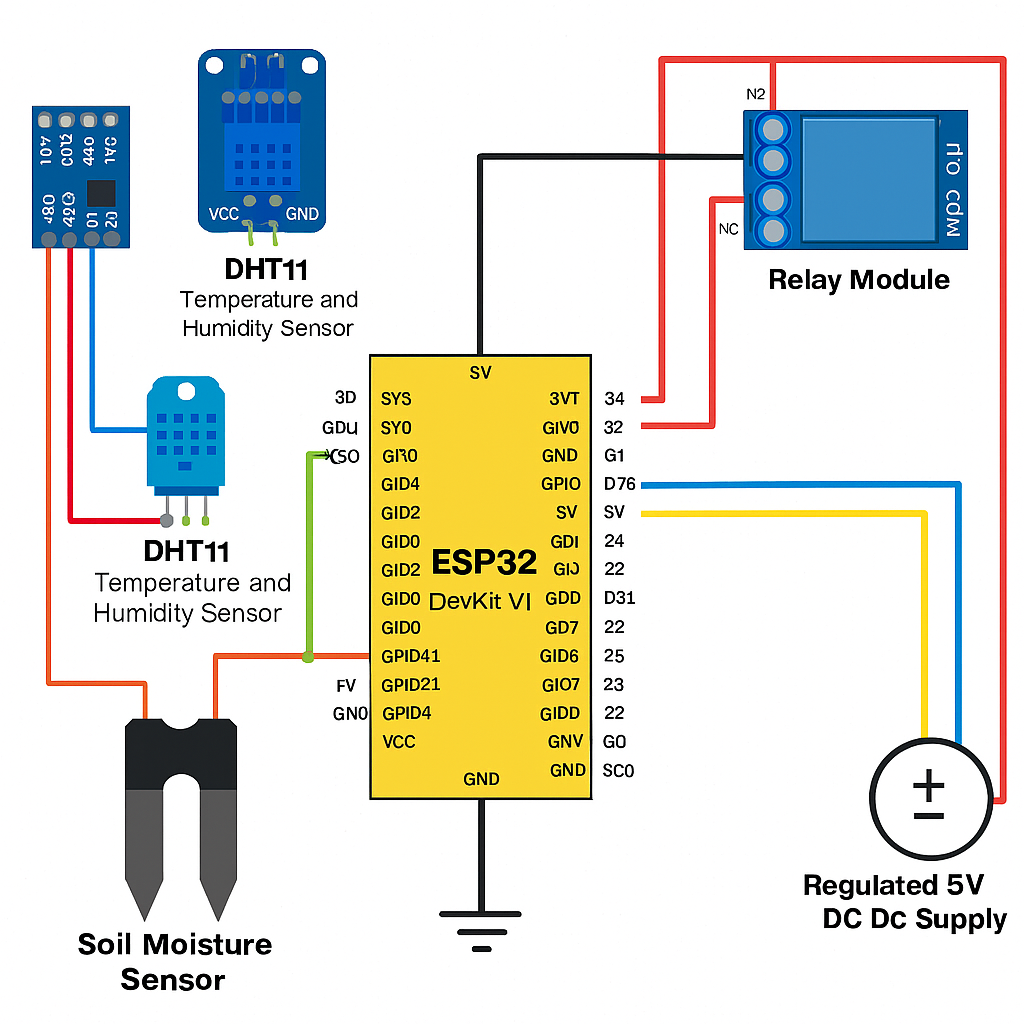
\includegraphics[width=0.85\textwidth]{image10.png}
    \caption{Sơ đồ cấu trúc phần cứng}
    \label{fig:hardware-diagram}
\end{figure}

\textbf{Bước 3: Lập trình firmware vi điều khiển}

Viết code khởi tạo phần cứng và logic kiểm soát bơm dựa trên các điều kiện
môi trường và dữ liệu kết quả từ ESP32-CAM.

\textbf{Bước 4: Thiết kế và lập trình giao diện}

Xây dựng các API thực hiện các chức năng: gửi yêu cầu đến ESP32-CAM lấy kết
quả nhận diện loại cây, quản lý thông tin người dùng, quản lý thông tin thiết
bị, gửi dữ liệu sau khi nhận diện đến ESP32 để thực hiện tưới cây. Thiết kế
giao diện trang web thân thiện, dễ sử dụng.

\textbf{Bước 5: Tích hợp và kiểm thử}

Kết nối toàn bộ hệ thống, kiểm thử các chức năng như chức năng nhận diện loại
cây, chức năng điều khiển máy bơm tự động, chức năng bật máy bơm thủ công,\ldots

% ============================================================
\section{Kết quả của đề tài}

\subsection{Giao diện trang web}

\begin{figure}[H]
    \centering
    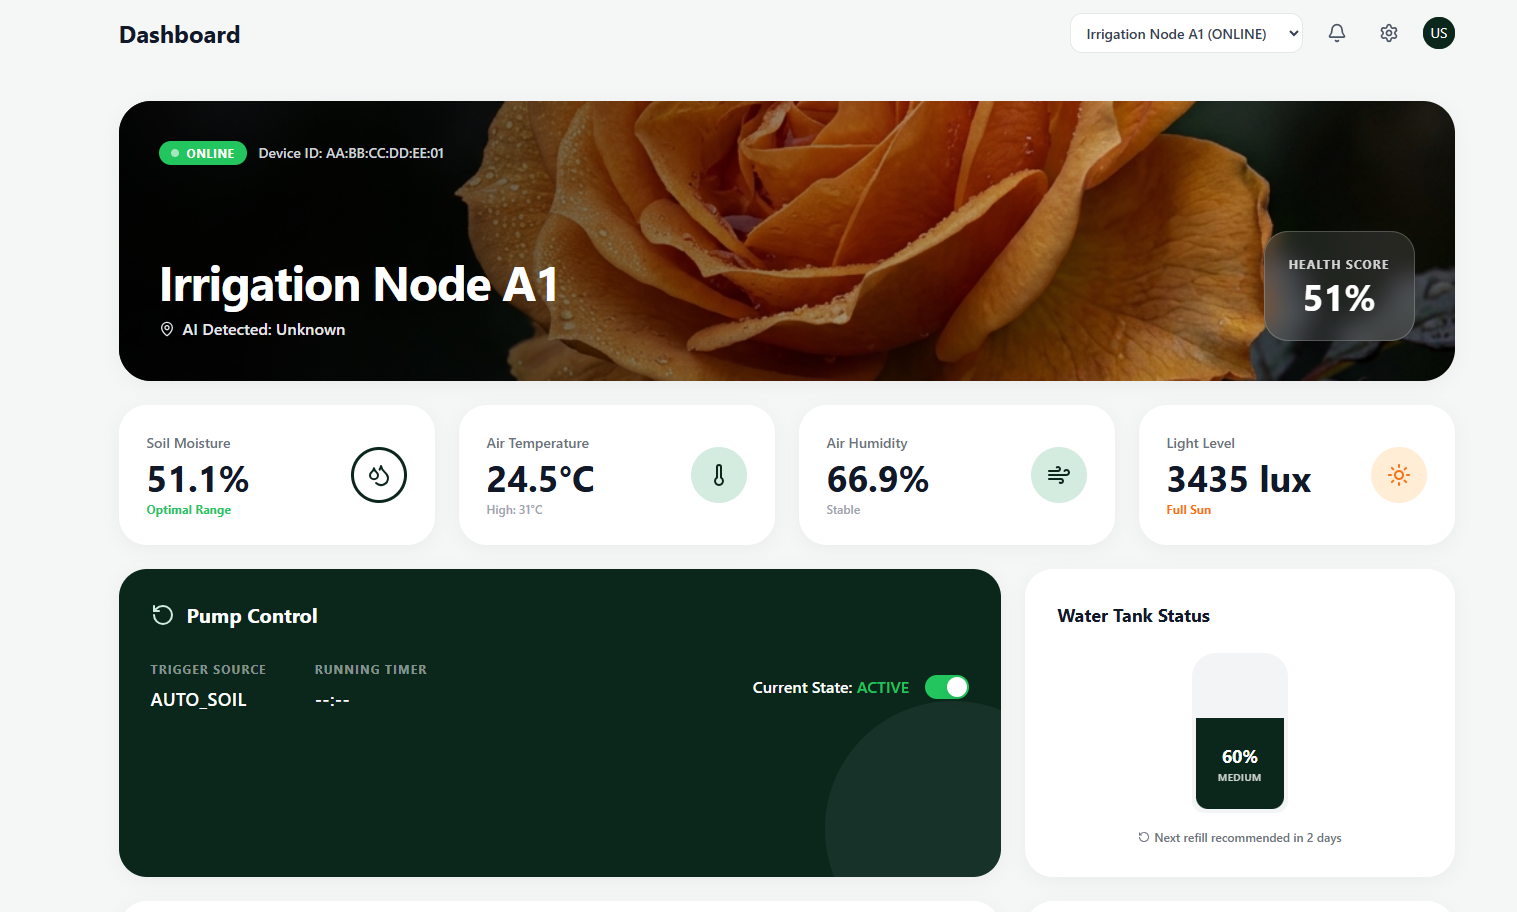
\includegraphics[width=0.9\textwidth]{image11.png}
    \caption{Giao diện dashboard}
    \label{fig:dashboard}
\end{figure}

Giao diện Dashboard đóng vai trò là trung tâm giám sát dữ liệu thời gian thực của hệ thống. Tại đây, người dùng có thể theo dõi trực quan các thông số môi trường quan trọng bao gồm:
\begin{itemize}
    \item \textbf{Thông số môi trường:} Độ ẩm đất (Soil Moisture), Nhiệt độ (Air Temperature), Độ ẩm không khí (Air Humidity).
    \item \textbf{Chỉ số sức khỏe cây trồng (Health Score):} Một thuật toán tổng hợp dựa trên các điều kiện môi trường để đánh giá trạng thái hiện tại của cây.
    \item \textbf{Điều khiển máy bơm (Pump Control):} Cho phép chuyển đổi linh hoạt giữa chế độ tự động (AUTO\_SOIL) và thủ công. Giao diện hiển thị trạng thái hoạt động hiện tại của bơm (Active/Inactive).
    \item \textbf{Trạng thái bồn chứa (Water Tank Status):} Hiển thị mức nước còn lại trong bình dựa trên dữ liệu từ cảm biến phao, kèm theo dự báo thời gian cần nạp thêm nước.
\end{itemize}

\begin{figure}[H]
    \centering
    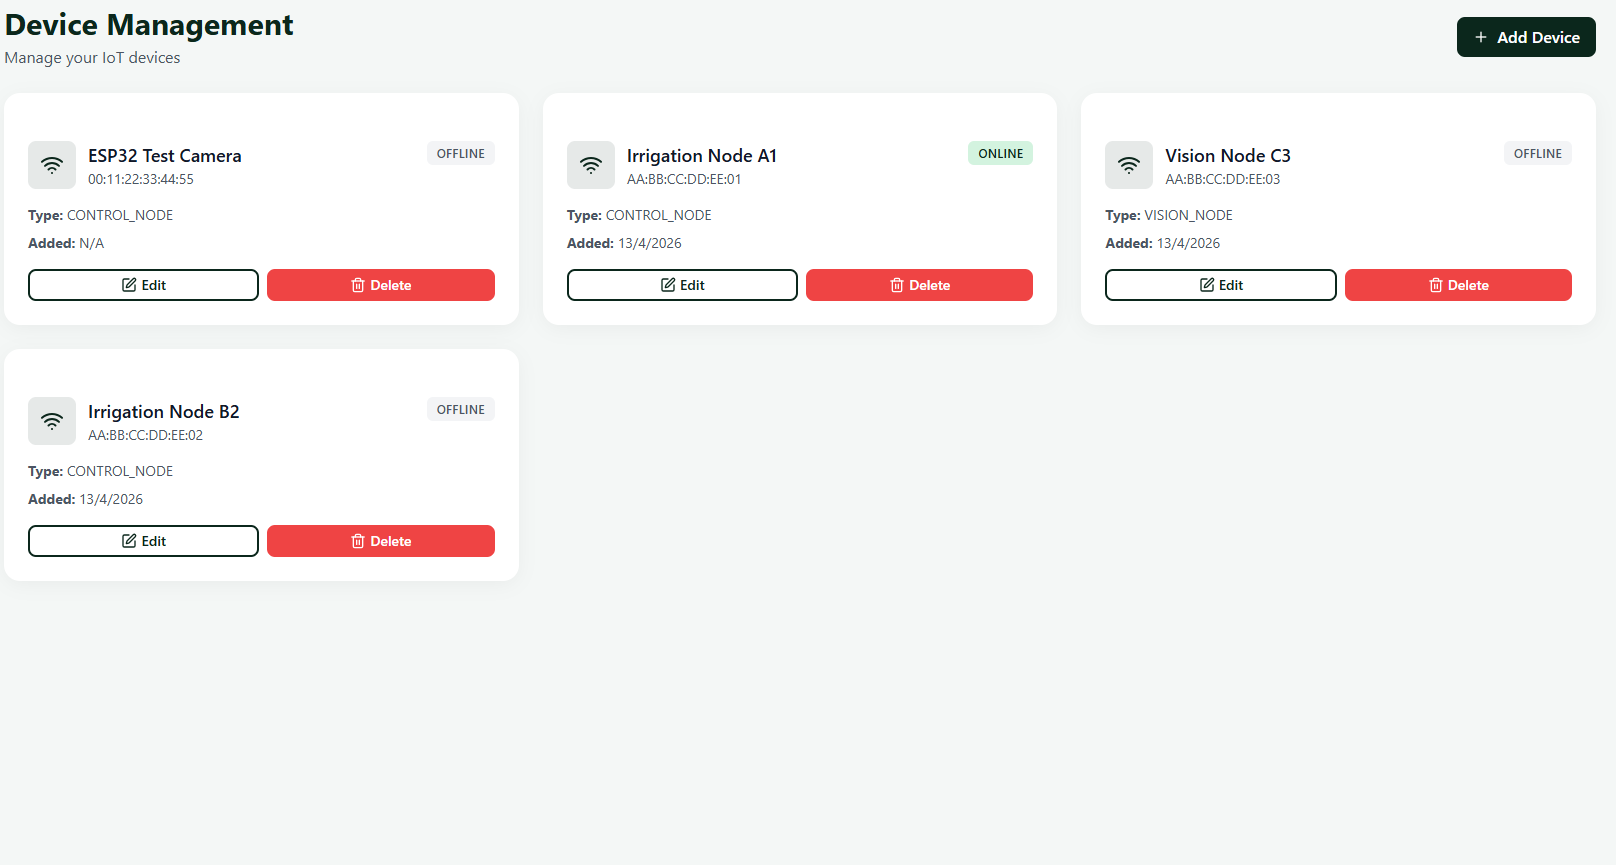
\includegraphics[width=0.9\textwidth]{image12.png}
    \caption{Giao diện quản lý thiết bị}
    \label{fig:device-management}
    \label{fig:device-management}
\end{figure}

Trang Quản lý thiết bị cho phép người dùng theo dõi và điều chỉnh danh sách các node IoT trong hệ thống:
\begin{itemize}
    \item \textbf{Danh sách thiết bị:} Hiển thị các card thông tin cho từng node như ESP32-CAM (Vision Node) và các node điều khiển (Control Node).
    \item \textbf{Trạng thái kết nối:} Hệ thống tự động cập nhật trạng thái Online hoặc Offline dựa trên tín hiệu Heartbeat gửi về máy chủ.
    \item \textbf{Thao tác quản lý:} Cung cấp các chức năng thêm mới thiết bị (Add Device), chỉnh sửa cấu hình hoặc xóa thiết bị khỏi hệ thống quản lý.
\end{itemize}

\begin{figure}[H]
    \centering
    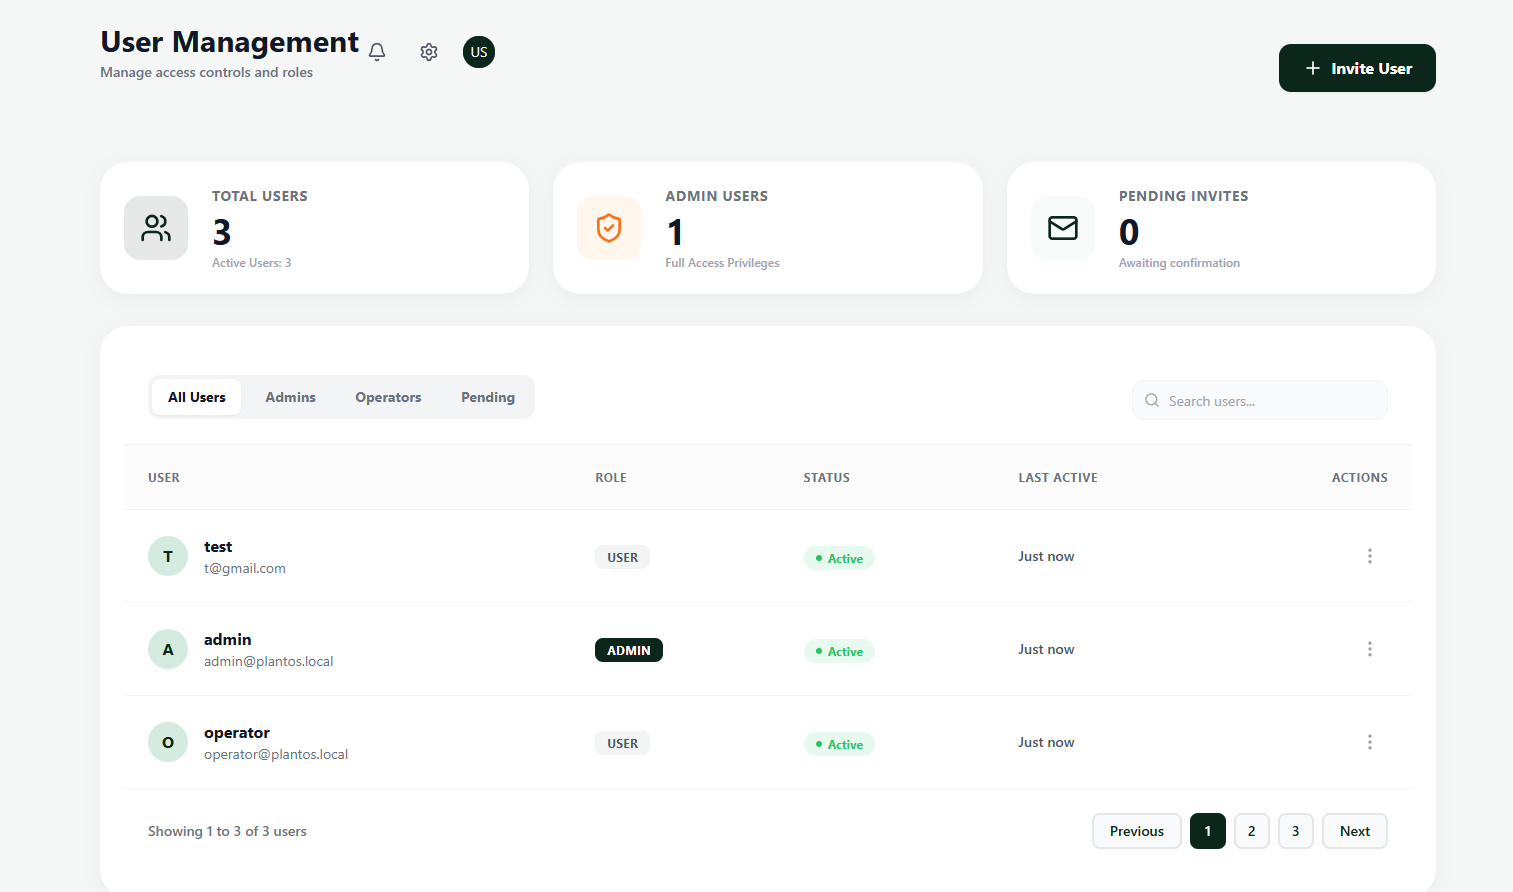
\includegraphics[width=0.9\textwidth]{image13.png}
    \caption{Giao diện quản lý người dùng}
    \label{fig:user-management}
\end{figure}

Giao diện Quản lý người dùng thể hiện tính năng phân quyền hệ thống sử dụng cơ chế JWT:
\begin{itemize}
    \item \textbf{Phân quyền vai trò (RBAC):} Hiển thị danh sách tài khoản với các vai trò cụ thể như ADMIN (toàn quyền) và USER (quyền giám sát).
    \item \textbf{Theo dõi hoạt động:} Ghi lại trạng thái hoạt động (Active) và thời điểm tương tác cuối cùng của từng thành viên.
    \item \textbf{Kiểm soát truy cập:} Quản trị viên có thể mời thêm người dùng mới hoặc điều chỉnh quyền hạn thông qua các nút thao tác nhanh trên danh sách.
\end{itemize}

\subsection{Đánh giá}

Đã thực hiện được các chức năng:

\begin{itemize}
    \item Nhận diện loại cây.
    \item Giám sát các thông số môi trường.
    \item Điều khiển máy bơm nước bật tắt theo yêu cầu hoặc tự động.
    \item Cảnh báo khi cạn nước.
    \item Mô hình AI có độ chính xác tương đối cao.
    \item Thời gian phản hồi dưới 7 giây.
\end{itemize}

% ============================================================
\chapter{KẾT LUẬN}
% ============================================================

\section{Những điểm đã đạt được của hệ thống}

\textbf{Về mặt hệ thống nhúng \& phần cứng:} Xây dựng thành công các node IoT
sử dụng vi điều khiển ESP32 và ESP32-CAM. Hệ thống đọc dữ liệu cảm biến (độ
ẩm đất, nhiệt độ, phao nước) theo thời gian thực với độ trễ thấp và điều
khiển máy bơm chính xác.

\textbf{Về mặt ứng dụng AI:} Triển khai thành công mô hình mạng nơ-ron học sâu
(Deep Learning) trực tiếp lên vi điều khiển ESP32-CAM có tài nguyên hạn chế
(TinyML). Mô hình có khả năng chụp ảnh và nhận diện loại cây ngay tại thiết bị
mà không cần đẩy ảnh lên cloud để xử lý, giúp giảm băng thông và độ trễ.

\textbf{Về mặt phần mềm \& Web Server:} Xây dựng kiến trúc Backend phân quyền
người dùng bảo mật với JWT. Giao diện Frontend trực quan, cho phép người dùng
giám sát thông số môi trường, xem kết quả AI nhận diện và điều khiển hệ thống
từ xa một cách thuận tiện.

\section{Những điểm chưa đạt được của hệ thống}

\textbf{Độ chính xác của AI phụ thuộc môi trường:} Mô hình nhận diện loại cây
hoạt động tốt trong điều kiện ánh sáng lý tưởng, nhưng tỷ lệ chính xác giảm
khi môi trường thiếu sáng, ngược sáng hoặc có quá nhiều chi tiết nhiễu.

\textbf{Công suất máy bơm hạn chế:} Máy bơm nước mini hiện tại chỉ có công suất
nhỏ, phù hợp cho mô hình chậu cây trồng trong nhà (indoor), chưa đủ áp lực
để triển khai thực tế cho một khu vườn rộng.

\textbf{Phụ thuộc vào mạng Wi-Fi:} Nếu mất kết nối Internet hoặc Server gặp sự
cố, tính năng cấu hình từ xa và nhận diện AI sẽ bị gián đoạn.

\section{Kết luận}

Nhóm đã hoàn thành mục tiêu ban đầu đặt ra là xây dựng thành công
\textbf{``Hệ thống tưới cây tự động thông minh tích hợp AI nhận diện loại
cây''}. Hệ thống không chỉ dừng lại ở việc tự động hóa tưới tiêu dựa trên cảm
biến đơn thuần, mà còn ứng dụng thành công công nghệ Trí tuệ nhân tạo tại biên
để cá nhân hóa việc chăm sóc cho từng loại cây cụ thể. Đề tài đã đáp ứng các
yêu cầu về cả phần cứng (thu thập dữ liệu, điều khiển chấp hành) và phần mềm
(xử lý dữ liệu, giao diện người dùng).

\section{Hướng phát triển}

\textbf{Tối ưu hóa giao thức IoT:} Chuyển đổi giao tiếp giữa thiết bị nhúng và
Server từ HTTP RESTful API sang giao thức MQTT để giảm overhead dữ liệu, tăng
tốc độ truyền tải hai chiều và tiết kiệm năng lượng hơn cho thiết bị IoT.

\textbf{Cải thiện AI và Thị giác máy tính:} Thu thập thêm tập dữ liệu hình ảnh
đa dạng (Data Augmentation) để huấn luyện (fine-tune) lại mô hình AI, giúp
nhận diện chính xác hơn ở các góc độ và điều kiện ánh sáng khác nhau. Tích hợp
thêm tính năng AI nhận diện bệnh tật trên lá cây.

\textbf{Tích hợp API Thời tiết:} Kết nối Backend với các API dự báo thời tiết bên
ngoài (như OpenWeatherMap). Nhờ đó, hệ thống có thể ra quyết định thông minh
hơn: ví dụ tự động hoãn lịch tưới nếu dự báo trời sắp mưa trong 2 giờ tới,
giúp tiết kiệm nước.

% ============================================================
\chapter*{TÀI LIỆU THAM KHẢO}
\addcontentsline{toc}{chapter}{TÀI LIỆU THAM KHẢO}
% ============================================================

\begin{enumerate}[label={[\arabic*]}]
    \item IoTZone, \textit{Giới thiệu ESP32 là gì?}, 2026. [Online]. Available: \url{https://iotzone.vn/esp32/esp32-co-ban/gioi-thieu-esp32-la-gi/}
    
    \item IMaker, \textit{Cảm biến độ ẩm đất điện dung}, 2026. [Online]. Available: \url{https://imaker.vn/cam-bien-do-am-dat}
    
    \item PLCTech, \textit{Relay là gì? Nguyên lý và cấu tạo}, 2026. [Online]. Available: \url{https://plctech.com.vn/relay-la-gi/}
    
    \item HShop, \textit{Động cơ bơm chìm Mini Water Pump 5VDC}, 2026. [Online]. Available: \url{https://hshop.vn/dong-co-bom-chim-mini-5vdc}
    
    \item NShop, \textit{Hướng dẫn sử dụng Module ESP32-CAM AI-Thinker}, 2026. [Online]. Available: \url{https://nshopvn.com/blog/gioi-thieu-mach-thu-phat-wifi-ble-esp32-cam-ai-
    thinker-huong-dan-su-dung-voi-arduino-thuc-hanh-lam-bo-mo-khoa-cua-nhan-
    dien-khuon-mat-bang-esp32-cam/}
    
    \item Caka, \textit{Phao cảm biến mực nước 52mm công tắc chất lỏng Mini ngang}, 2026. [Online]. Available: \url{https://caka.vn/phao-cam-bien-muc-nuoc-52mm-cong-tac-chat-long-mini-ngang}
    
    \item Studocu, \textit{Nguyên lý hoạt động cảm biến nhiệt độ, độ ẩm DHT11}, 2026. [Online]. Available: \url{https://www.studocu.vn/vn/document/vnu-university-of-engineering-and-technology/nguyen-ly-ky-thuat-dien-tu/dht11-thank-you/111744380}
\end{enumerate}

\end{document}